\chapter{Исследовательский раздел}

В данном разделе будут представлены технические характеристики и будет проведено исследование.

\section{Технические характеристики}
Технические характеристики устройства, на котором выполнялось исследование:
\begin{itemize}
	\item операционная система: Ubuntu 20.04~\cite{ubuntu};
	\item размер оперативной памяти: 16 Гбайт;
	\item процессор AMD Ryzen 5 5500U with Radeon Graphics.

\end{itemize}
	
На протяжении всего тестирования компьютер был подключен к сети питания.
\section{Исследование}
Задача заключалась в исследования зависимости времени работы от сложности запроса.
Исследование проводилось на заранее заготовленной таблице, количество записей в которой было равно 500 штук.

Градация сложности запросов была следующая:
\begin{enumerate}
	\item запрос первой сложности:
		\begin{lstlisting}[language=sql, label=lst:query_1]
		select equipment.id from equipment\end{lstlisting}
	\item запрос второй сложности:
		\begin{lstlisting}[language=sql, label=lst:query_2]
		select equipment.id,
			equipment.name,
			equipment.type,
			equipment.studio_id
		from equipment\end{lstlisting}
	\item запрос третьей сложности:
		\begin{lstlisting}[language=sql, label=lst:query_2]
		select equipment.id,
			equipment.name,
			equipment.type,
			equipment.studio_id
		from equipment where 
			equipment.studio_id = $1\end{lstlisting}
	\item запрос четвертой сложности:
		\begin{lstlisting}[language=sql, label=lst:query_2]
		select equipment.id,
			equipment.name,
			equipment.type,
			equipment.studio_id
		from equipment where 
			equipment.studio_id = $1 and
			equipment.type = $2\end{lstlisting}
	\item запрос пятой сложности
			\begin{lstlisting}[language=sql, label=lst:query_2]
			select equipment.id,
				equipment.name,
				equipment.type,
				equipment.studio_id
			from equipment where 
				equipment.studio_id = $1 and
				equipment.type = $2 and 
				not exists
					(select * from reserved_equipments where equipment.id = reserved_equipments.equipment_id)\end{lstlisting}
	\item запрос шестой сложности
			\begin{lstlisting}[language=sql, label=lst:query_2]
			select equipment.id, 
				equipment.name,
				equipment.type,
				equipment.studio_id,
				to_char(reserve.start_time, 'YYYY-MM-DD HH24:MI:SS'),
				to_char(reserve.end_time, 'YYYY-MM-DD HH24:MI:SS')
			from equipment, reserve where 
				equipment.studio_id = $1 and 
				equipment.type = $2 and 
				exists 
					(select * from reserved_equipments where equipment.id = reserved_equipments.equipment_id)\end{lstlisting}
\end{enumerate}  

Для каждого запроса время замерялось 1000 раз и суммировалось.
После чего бралось среднее значение.

По итогам исследования получились следующие результаты, представленные в таблице~\ref{table:res} и на рисунке~\ref{img:chart}.

\begin{table}[h]

	\centering
	\begin{tabular}{ | c | c | }
		\hline
		Уровень сложности запроса & Время работы, мс \\ \hline
		1 & 1.181 \\
		2 & 1.383 \\
		3 & 1.397 \\
		4 & 1.402 \\
		5 & 1.445 \\
		6 & 1.532 \\
		\hline
	\end{tabular}
	\caption{Результаты исследования}
				\label{table:res}
\end{table}


\begin{center}
	\centering
	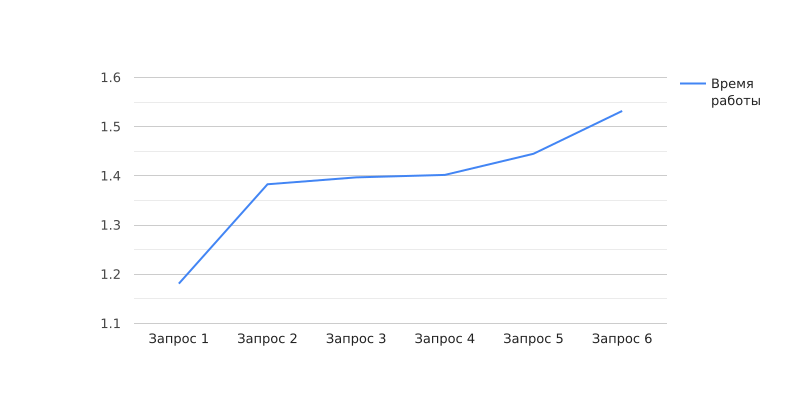
\includegraphics[height=0.3\textheight]{inc/img/chart.png}
	\captionof{figure}{График зависимости времени работы от сложности запроса}
	\label{img:chart}
\end{center}
\section*{Вывод}
В ходе выполнения исследовательской части было выявлено, что время работы напрямую зависит от сложности запроса --- чем сложнее запрос, тем больше времени системе требуется на его обработку.
Также на графике можно наблюдать довольно резкий скачок времени работы в 1.16 раз между Запросом 1 и Запросом 2.
Это можно объяснить тем, что в инструкции SELECT Запроса 1 необходимо вернуть одно значение, а в инструкции SELECT Запроса 2 4 значения.
При проходе по всей таблице, системе необходимо вернуть ответ, который будет включать в себя больше значений, чем при Запросе 1.
Также большое время при выполнении Запроса 6 можно объяснить работой с двумя таблицами.

 